%%% Local Variables:
%%% mode: latex
%%% TeX-master: "report_main"
%%% End:

\section{Part 1 - Mathematical modeling}
\subsection{Problem 1}

We use the helicopter model \cref{fig:helicopter_model} as our starting point for deriving the equations of motion.
\begin{figure}[hbp]
\caption{the helicopter model figure 7 from the assignment \cite[p.12]{assignment} with relevant distances drawn in.}
\label{fig:helicopter_model}
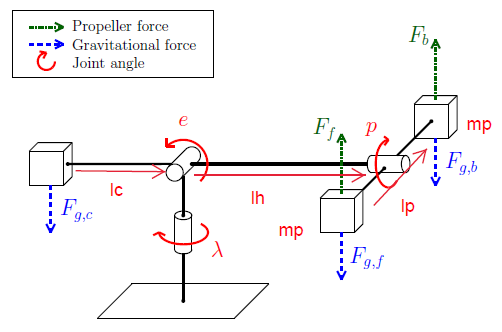
\includegraphics[width=\textwidth]{images/helicopter_model}
\end{figure}

The equations of motion for the pitch is the momentum around the point p in the clockwise direction as shown in \cref{fig:helicopter_model}:
\begin{align*}
J_p\ddot{p} &= l_p(F_{g,b} - F_b - F_{g,f} + F_f) \\
						&= l_p(m_pg - mp_g + K_fV_f - V_b) \\
						&= l_pK_f(V_f-V_b)
\end{align*}
Since $V_d = V_f-V_b$, we can write this as:
\begin{equation}
J_p\ddot{p} = l_pK_fVd
\end{equation}
Here, we can see that $L_1 = l_pK_f$.

\begin{figure}[H]
\caption{the elevation model}
\label{fig:elevation_model}
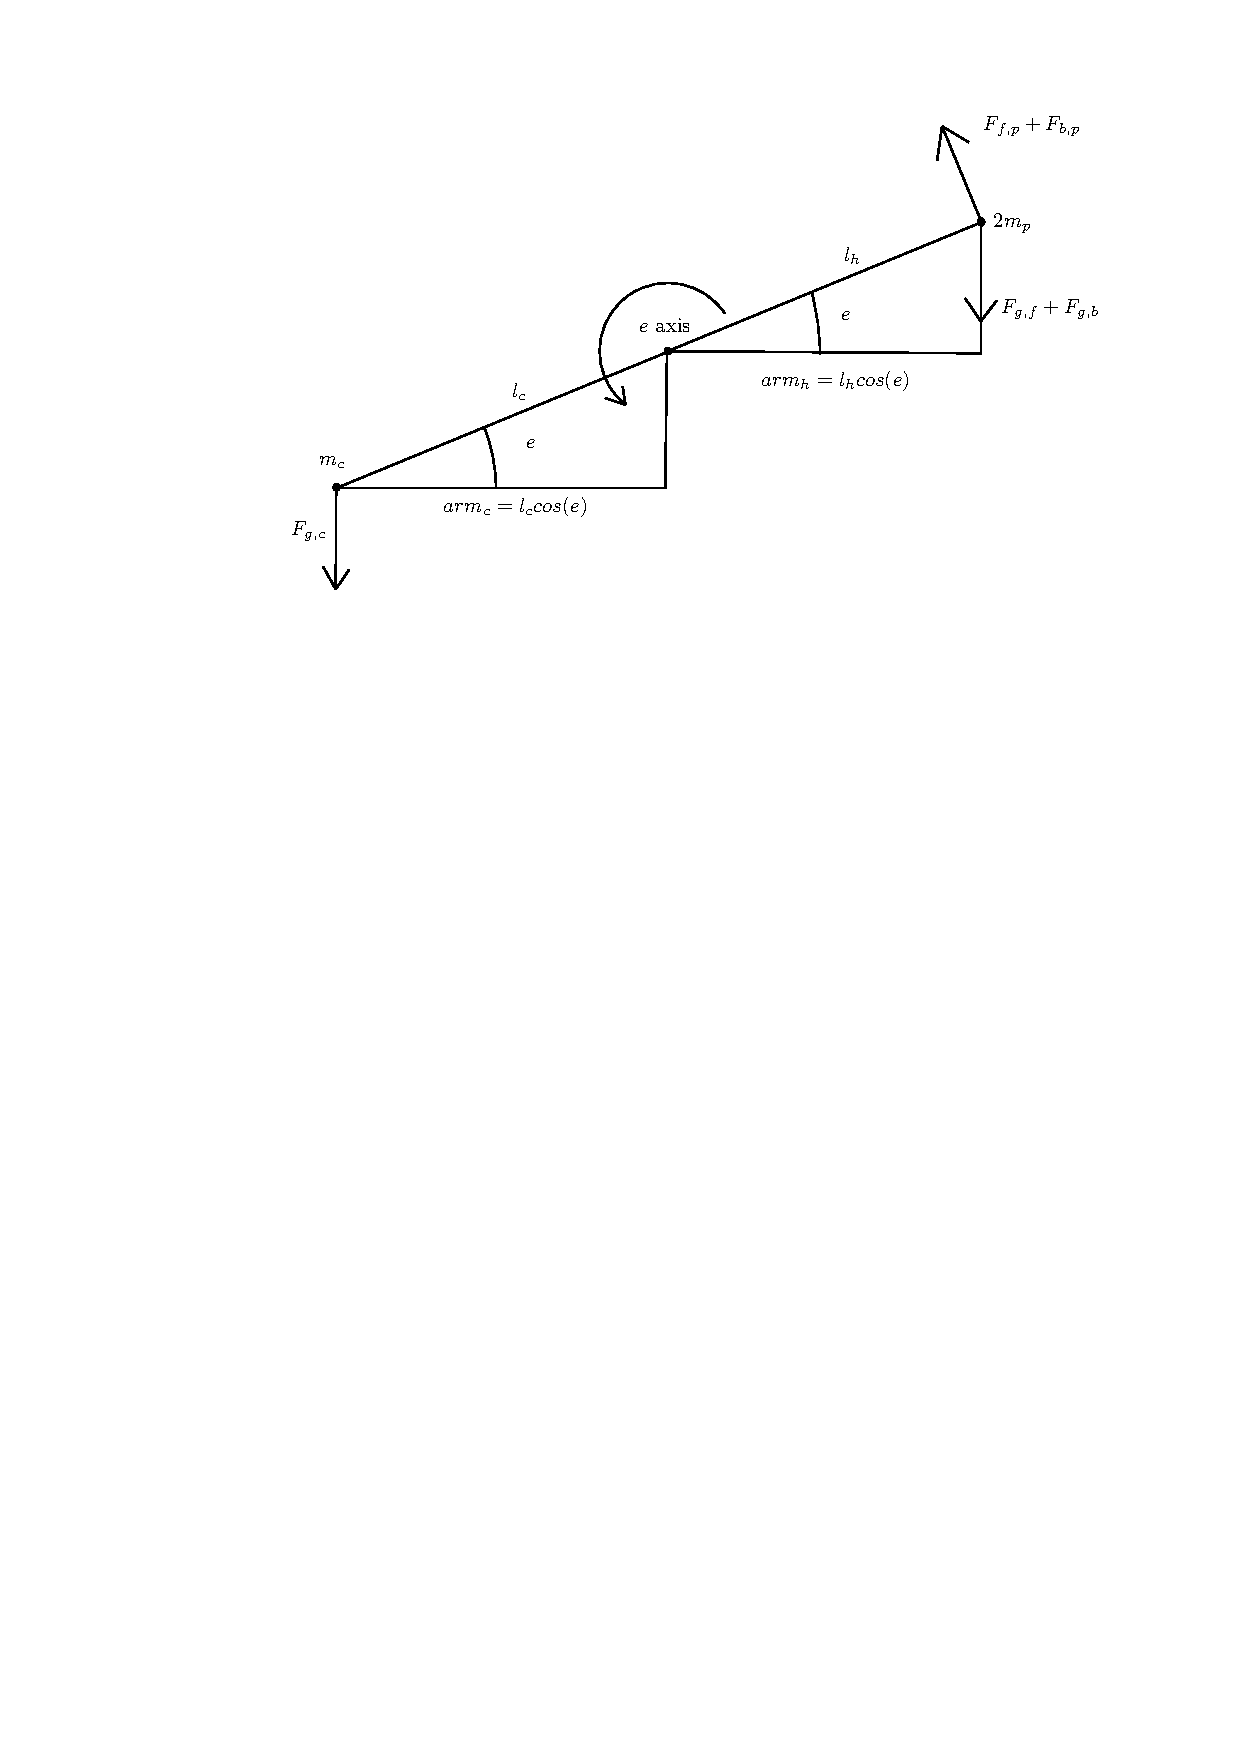
\includegraphics[width=0.5\textwidth]{images/elevation_model}
\end{figure}

\subsection{Problem 2}
\subsection{Problem 3}
\subsection{Problem 4}
